\documentclass[conference]{IEEEtran}
\IEEEoverridecommandlockouts

\usepackage{cite}
\usepackage{amsmath,amssymb}
\usepackage{graphicx}
\usepackage{textcomp}
\usepackage{xcolor}
\usepackage{url}
\usepackage{tikz}
\usetikzlibrary{shapes.geometric, arrows.meta, positioning}

% ======================================================================
% HOW THIS FILE WORKS (read before editing)
%  * Sections I-III are the Review-1 paper, carried over in the team's
%    own words. Lines marked "% FIX:" say what is no longer true.
%    Material marked \iffalse ... \fi is Review-1 text kept for reuse;
%    it does not print.
%  * Sections IV-VII are new. Each red [WRITE ...] marker in the PDF is a
%    place for the team's own sentences. The "% FACT:" lines under it are
%    the verified numbers and where each comes from. They never print.
%  * Every table and Fig. 2 are generated from the results files by
%    report/paper/build_assets.py; do not retype numbers by hand.
%  * Delete every \WRITE{...} marker before submitting.
% ======================================================================
\newcommand{\WRITE}[1]{{\color{red}\textbf{[WRITE: #1]}}}

\def\BibTeX{{\rm B\kern-.05em{\sc i\kern-.025em b}\kern-.08em
    T\kern-.1667em\lower.7ex\hbox{E}\kern-.125emX}}

\begin{document}

\title{IndicBridge: Investigating Linguistic Relatedness in\\
Cross-Lingual Multistage Fine-Tuning of Whisper for\\
Low-Resource Indic Speech Recognition}

% FIX: check the spelling of every name before submitting.
\author{
\IEEEauthorblockN{Gourab Dash}
\IEEEauthorblockA{\textit{School of Computer Science and Engineering}\\
\textit{RV University}, Bengaluru, India\\
1RUA24CSE0146}
\and
\IEEEauthorblockN{Parth Nandkumar Khandagale}
\IEEEauthorblockA{\textit{School of Computer Science and Engineering}\\
\textit{RV University}, Bengaluru, India\\
1RUA24CSE0201}
\and
\IEEEauthorblockN{Divyansh Mahecha}
\IEEEauthorblockA{\textit{School of Computer Science and Engineering}\\
\textit{RV University}, Bengaluru, India\\
1RUA24CSE0139}
\and
\IEEEauthorblockN{Kaushal BC}
\IEEEauthorblockA{\textit{School of Computer Science and Engineering}\\
\textit{RV University}, Bengaluru, India\\
1RUA24CSE0196}
}

\maketitle

\begin{abstract}
\WRITE{abstract, about 170 words, in your own words. The Review-1 abstract
described a literature review; this one must state what was done and found.}
% Structure: problem (1 sentence) -> what you did (2) -> main result with
% numbers (2-3) -> other findings (2) -> what it means (1).
% FACT: 25 runs; whisper-base (74M) + LoRA; Hindi and English pivots of equal
%       size (45 h each); targets Marathi, Odia (Indo-Aryan), Kannada
%       (Dravidian), 15 h each; two test sets (FLEURS test, Kathbath valid,
%       600 clips each).                       [results/results_master.csv]
% FACT: Hindi pivot gain over direct training, WER points, FLEURS / Kathbath:
%       Marathi +3.1 / +3.5, Odia +3.1 / +1.9, Kannada +1.1 / +0.8 (Kathbath
%       interval includes zero).               [results/tables/gains.csv]
% FACT: English pivot of the same size never gives a significant gain; it
%       hurts Kannada on FLEURS (-1.3, CI -2.4 to -0.4).        [gains.csv]
% FACT: Hindi pivot beats English pivot for all three targets on both test
%       sets: Marathi +3.0 / +4.6, Odia +3.1 / +2.6, Kannada +2.5 / +1.9.
% FACT: Indo-Aryan-only extra benefit is not consistent: only Marathi vs
%       Kannada on Kathbath (+2.7, CI 1.0 to 4.8). [results/tables/interaction.csv]
% FACT: Odia: 3.09 Whisper tokens per letter vs 1.29 for Hindi; 23.1% of
%       FLEURS Odia sentences exceed the decoder limit; untrained output is
%       0% Odia script; borrowed token (Bengali/Assamese/Hindi) makes no
%       reliable difference after training.     [Table VI]
% FACT: fp16 MLX model, 144 MB, runs at RTF 0.03-0.06 on an Apple M4.
% DO NOT CLAIM: "language family drives transfer" -- the data says
%       relatedness helps but the family-specific extra is not established.
\end{abstract}

\begin{IEEEkeywords}
Automatic Speech Recognition, Low-Resource Languages, Cross-Lingual
Transfer, Multistage Fine-Tuning, Whisper, LoRA, Parameter-Efficient
Fine-Tuning, Indic Languages, Odia, Word Error Rate.
\end{IEEEkeywords}

% ======================================================================
\section{Introduction}
% Carried over from Review-1. Reword in your team's voice: Turnitin's AI
% check runs on the whole paper, these sections included.

\subsection{Background and Context}

Automatic speech recognition has undergone a substantial architectural
shift over the past five years. Early neural ASR systems were trained
per language on curated transcribed corpora, which limited coverage to
languages with substantial annotated data. Self-supervised learning
changed this by enabling representation learning from unlabelled audio,
with wav2vec 2.0 and its cross-lingual successors XLSR-53 and XLS-R
demonstrating that a single model pre-trained on many languages could be
fine-tuned to individual languages with comparatively little labelled
data \cite{conneau2021xlsr, babu2022xlsr}.

A parallel direction pursued scale through weak supervision rather than
self-supervision. Whisper was trained on 680{,}000 hours of loosely
labelled multilingual audio scraped from the web and performs
transcription, translation, language identification and voice activity
detection within a single encoder--decoder Transformer \cite{radford2023whisper}.
Its practical appeal lies in requiring no fine-tuning for
high-resource languages. Massively Multilingual Speech (MMS) extended
coverage further, scaling recognition to over one thousand languages
\cite{pratap2024mms}.

Coverage, however, is not the same as competence. Whisper's training
distribution is heavily skewed toward English and a small number of
European languages, and its reported error rates vary by more than an
order of magnitude across its supported set \cite{radford2023whisper}.
For most Indian languages the model is nominally supported but
practically unusable without adaptation. This motivated a body of work
on efficiently adapting large pre-trained speech models to
under-represented languages.

\subsection{Motivation and Research Gap}

The motivation for IndicBridge arises from a specific unverified claim.
The multistage fine-tuning result is explained by its authors in terms
of linguistic relatedness: Tamil helps Malasar because the two are
related Dravidian languages \cite{pillai2024multistage}. This is a
plausible and intuitive explanation, but the study evaluated exactly one
pivot--target pair. No unrelated pivot was tested. Consequently the
observed improvement is equally consistent with a simpler alternative
explanation---that any additional in-domain Indian speech data
would have produced a comparable benefit, regardless of family
membership.

Distinguishing these two explanations is not a matter of academic
tidiness. It determines practical guidance for the many Indian languages
still lacking usable ASR. If relatedness is the operative mechanism,
practitioners should select pivots by language family. If data quantity
dominates, practitioners should simply select the largest available
Indic corpus. The two prescriptions diverge sharply for Dravidian
languages, for which the largest available Indian corpora are
Indo-Aryan.

Suggestive evidence exists on both sides. Rouditchenko \emph{et al.}\
report that pre-training hours \emph{per language family} carry
predictive power, which favours the relatedness account
\cite{rouditchenko2023unseen}. Song \emph{et al.}\ observe that
similarity between languages can be exploited through LoRA
initialization when extending multilingual ASR to new languages
\cite{song2024lorawhisper}. Neither study, however, isolates relatedness
as an independent variable while holding data quantity, model size, and
optimization budget fixed.

% Review-1 "Current Research Landscape" -- removed to fit 6 pages; Section II covers it.
\iffalse
Research relevant to this problem can be organized into five strands.
The first established multilingual speech representations through
self-supervision \cite{conneau2021xlsr, babu2022xlsr} and weak
supervision \cite{radford2023whisper, pratap2024mms}. The second
examined how such models behave on languages absent from pre-training,
with Rouditchenko \emph{et al.}\ fine-tuning both XLS-R and Whisper on
thirteen unseen and eighteen seen languages and finding that the number
of pre-training hours seen per language \emph{and per language family}
predicts comparative performance \cite{rouditchenko2023unseen}. The
third strand introduced sequential and multistage transfer for extremely
low-resource targets \cite{pillai2024multistage}. The fourth developed
parameter-efficient adaptation for speech models
\cite{hu2022lora, song2024lorawhisper, xu2024rehearsalfree, ferraz2024distilwhisper}.
The fifth constructed Indic-specific corpora, benchmarks and systems
\cite{bhogale2023vistaar, javed2024indicvoices, javed2023indicsuperb,
conneau2023fleurs, ardila2020commonvoice}.
\fi

% ======================================================================
\section{Literature Review}
% Carried over from Review-1. PAGE BUDGET: this section should end up at
% about 650 words (it is about 1,250 now) to keep the paper at 6 pages.

The literature is organized thematically, tracing the development from
multilingual representation learning toward controlled, efficient, and
correctly evaluated low-resource adaptation.

\subsection{Multilingual Speech Representation Learning}

Conneau \emph{et al.}\ introduced XLSR-53, extending wav2vec 2.0 to
cross-lingual self-supervised pre-training over 53 languages, and
demonstrated that a shared quantized latent space learned across
languages improves recognition for individual low-resource languages
relative to monolingual pre-training \cite{conneau2021xlsr}. XLS-R
subsequently scaled this approach to 128 languages and up to two billion
parameters, reporting gains across recognition, translation and
classification \cite{babu2022xlsr}.

These works established the central premise on which our study rests:
representations learned from one set of languages transfer usefully to
others. What they did not resolve is which source languages transfer
best to a given target, since transfer was studied in aggregate rather
than pairwise.

\subsection{Weakly-Supervised Multilingual ASR}

Whisper represents an alternative scaling philosophy \cite{radford2023whisper}.
Rather than self-supervised pre-training followed by supervised
fine-tuning, Whisper is trained end-to-end on a very large,
weakly-labelled and noisy multilingual corpus. The resulting model
generalizes robustly in a zero-shot setting for well-represented
languages.

Two properties of Whisper are directly consequential for our work. The
first is the fixed language-token vocabulary. Whisper conditions
decoding on a discrete language token drawn from a closed set of 99
languages. Inspection of the official tokenizer
implementation\footnote{Verified against the \texttt{LANGUAGES}
dictionary in \texttt{whisper/tokenizer.py} in the official OpenAI
repository. The claim is directly reproducible:
\texttt{grep -E '"(as|bn|hi|kn|mr|or)":' whisper/tokenizer.py} returns
entries for all listed codes except \texttt{or}.} confirms
that Bengali (\texttt{bn}), Hindi (\texttt{hi}), Kannada (\texttt{kn}),
Marathi (\texttt{mr}) and Assamese (\texttt{as}) are present, whereas
\textbf{Odia possesses no language token}. The second is the byte-level
BPE tokenizer, which can encode arbitrary Unicode text---including Odia
script---but at a substantially higher token-per-word cost for scripts
absent from the training distribution.

The combination of these two properties makes Odia an unusually
informative test case: it is a genuinely unseen language for a model
that nominally covers South Asia, spoken by a population large enough
that the omission carries real consequence.

MMS pursued breadth explicitly, scaling to more than one thousand
languages by combining self-supervised pre-training with religious-text
recordings for supervision \cite{pratap2024mms}. It demonstrates that
coverage can be extended dramatically, while also illustrating that
domain-restricted supervision constrains the resulting model's
generality.

\subsection{Adaptation to Languages Unseen During Pre-Training}

The most directly relevant empirical study is that of Rouditchenko
\emph{et al.}, who compare XLS-R and Whisper when fine-tuned on
thirteen languages unseen during pre-training and eighteen seen
languages \cite{rouditchenko2023unseen}. Their central finding is that
the number of pre-training hours observed per language, and per language
family, predicts which model adapts better---despite the substantial
methodological differences between self-supervised and weakly-supervised
pre-training.

This result is important for two reasons. It confirms that unseen
languages are a distinct regime rather than merely a harder version of
the seen-language case, and it provides the strongest existing evidence
that \emph{family-level} exposure matters. However, the study measures
family exposure during pre-training as an observational covariate. It
does not manipulate the family relationship of an intermediate
fine-tuning stage experimentally, which is precisely the intervention
our work proposes.

\subsection{Sequential and Multistage Transfer}

Pillai \emph{et al.}\ propose multistage fine-tuning as a strategy for
languages with essentially no digital resources \cite{pillai2024multistage}.
Malasar, a Dravidian language of the Western Ghats spoken by
approximately ten thousand people, has no native script; the authors
therefore collected a spoken corpus transcribed in Tamil script in
collaboration with Wycliffe India and the speaker community. Rather than
fine-tuning Whisper directly on this small corpus, they first obtain an
intermediate Tamil ASR model---using both small and medium Whisper
architectures---and subsequently fine-tune that intermediate model on
Malasar.

The reported outcome is a WER of 51.9\%, representing a 4.5\% absolute
reduction relative to direct fine-tuning, with a further reduction to
47.3\% following punctuation removal in post-processing
\cite{pillai2024multistage}.

Three observations follow. First, the method is genuinely effective and
computationally modest, making it well suited to student and
resource-constrained research. Second, the post-processing gain of 4.6\%
absolute exceeds the gain from the proposed method itself, which
indicates that evaluation methodology for Indic-script ASR is
insufficiently standardized. Third---and central to our contribution---the
causal explanation offered for the method is untested. The study
compares multistage against direct fine-tuning, but does not compare
\emph{related} against \emph{unrelated} pivots.

\subsection{Parameter-Efficient Adaptation}

LoRA reparameterizes weight updates as low-rank matrices, freezing the
pre-trained backbone and training a small number of additional
parameters \cite{hu2022lora}. Adapter-based transfer established the
broader principle earlier for language models
\cite{houlsby2019adapters}, and MAD-X applied it specifically to
cross-lingual transfer through separable language and task adapters
\cite{pfeiffer2020madx}.

Within speech, Song \emph{et al.}\ propose LoRA-Whisper, incorporating
LoRA matrices into Whisper for multilingual ASR
\cite{song2024lorawhisper}. They report that the approach mitigates
language interference and that exploiting similarities between languages
through LoRA enables better performance on newly added languages while
preserving performance on existing ones. Xu \emph{et al.}\ pursue a
related objective, presenting a LoRA-based case study on Whisper aimed
at rehearsal-free multilingual extension \cite{xu2024rehearsalfree}.
Ferraz \emph{et al.}\ take a complementary distillation route with
Multilingual DistilWhisper, using language-specific experts to retain
per-language capability in a smaller model
\cite{ferraz2024distilwhisper}.

% FIX: the next sentence says "free-tier GPU quotas" -- the study actually
% ran on one Apple M4 laptop (16 GB). Also "ten-configuration" -> 25 runs.
For our purposes, parameter-efficient adaptation is enabling rather than
novel. It makes a ten-configuration comparative study feasible within
free-tier GPU quotas, and---because LoRA adapters are composable and
small---it makes multistage chaining operationally simple. The residual
question these works leave open is whether the observed benefit of
"language similarity" is linguistic or merely statistical.

\subsection{Indic Speech Resources and Systems}

AI4Bharat has produced the principal open resources for Indian language
speech. IndicVoices is a dataset of natural and spontaneous speech
totalling 23.7K hours from 51K speakers across more than 400 districts
and 22 languages, comprising read, extempore and conversational audio
\cite{javed2024indicvoices}. IndicSUPERB introduced the Kathbath corpus
and an evaluation suite for Indian language speech processing
\cite{javed2023indicsuperb}.

Bhogale \emph{et al.}\ contribute Vistaar, a collection of 59 benchmarks
across language and domain combinations, and train IndicWhisper by
fine-tuning Whisper on 10.7K hours across 12 Indian languages
\cite{bhogale2023vistaar}. IndicWhisper achieves the lowest WER on 39 of
the 59 benchmarks, with an average reduction of 4.1 WER points. The
authors further demonstrate that model rankings vary considerably across
benchmarks, so that comparisons drawn from a single benchmark may be
weakly correlated with those drawn from another.

% FIX: the second test set used was Kathbath, not Common Voice (Common
% Voice left the Hugging Face hub in Oct 2025). Keep the Common Voice
% citation if you mention why it was replaced.
This last finding directly shapes our evaluation design and motivates
our use of two independent test sets. FLEURS provides parallel read
speech across 102 languages and is widely adopted for cross-lingual
comparison \cite{conneau2023fleurs}, while Common Voice supplies
volunteer-recorded speech under markedly different acoustic conditions
\cite{ardila2020commonvoice}.

Notably, IndicWhisper is trained jointly across languages rather than
sequentially, and therefore does not isolate pairwise transfer effects.

\subsection{Evaluation and Optimization Under Data Imbalance}

Pi\~{n}eiro-Mart\'{i}n \emph{et al.}\ examine multilingual ASR training
under language imbalance, proposing weighted cross-entropy to improve
low-resource language performance within a multilingual model
\cite{pineiro2024weighted}. Their work reinforces a theme running
through this review: when languages differ substantially in available
data, both the optimization objective and the evaluation protocol
require deliberate design rather than default settings.

\subsection{Comparative Analysis}

Table~\ref{tab:comparison} summarizes the reviewed studies by method,
evaluation setting, principal finding, and limitation with respect to
our research question.

\begin{table*}[!t]
\caption{Comparative Analysis of the Reviewed Studies}
\label{tab:comparison}
\centering
\renewcommand{\arraystretch}{1.2}
\scriptsize
\begin{tabular}{|p{2.4cm}|p{3.1cm}|p{3.0cm}|p{3.6cm}|p{3.6cm}|}
\hline
\textbf{Study} & \textbf{Method / Model} & \textbf{Dataset / Evaluation} &
\textbf{Key Finding} & \textbf{Key Limitation} \\
\hline
Conneau \emph{et al.} \cite{conneau2021xlsr} &
XLSR-53, cross-lingual wav2vec 2.0 &
CommonVoice, BABEL &
Shared cross-lingual representations outperform monolingual pre-training. &
Transfer studied in aggregate; no pairwise source--target analysis. \\
\hline
Babu \emph{et al.} \cite{babu2022xlsr} &
XLS-R, up to 2B parameters, 128 languages &
Multiple ASR and translation benchmarks &
Scaling cross-lingual self-supervision improves low-resource ASR. &
Very large compute requirement; family effects not isolated. \\
\hline
Radford \emph{et al.} \cite{radford2023whisper} &
Whisper, weakly-supervised encoder--decoder &
680K hours, multilingual zero-shot evaluation &
Large-scale weak supervision yields robust zero-shot ASR. &
Closed 99-language token set; Odia absent; highly uneven per-language quality. \\
\hline
Pratap \emph{et al.} \cite{pratap2024mms} &
MMS, 1000+ language ASR &
Multilingual recognition and identification &
Language coverage can be extended by an order of magnitude. &
Supervision drawn from a narrow domain; limited generality. \\
\hline
Rouditchenko \emph{et al.} \cite{rouditchenko2023unseen} &
Fine-tuning XLS-R vs.\ Whisper &
13 unseen and 18 seen languages &
Pre-training hours per language and per family predict adaptation quality. &
Family exposure is observational, not experimentally manipulated. \\
\hline
Pillai \emph{et al.} \cite{pillai2024multistage} &
Multistage fine-tuning, Whisper via Tamil pivot &
Malasar corpus ($\approx$4h36m) &
51.9\% WER, 4.5\% absolute gain over direct fine-tuning; 47.3\% after punctuation removal. &
Single pivot--target pair; relatedness claim untested against an unrelated control. \\
\hline
Hu \emph{et al.} \cite{hu2022lora} &
LoRA low-rank adaptation &
NLP transfer benchmarks &
Comparable quality while training under 1\% of parameters. &
Not originally evaluated for speech or cross-lingual transfer. \\
\hline
Houlsby \emph{et al.} \cite{houlsby2019adapters} &
Bottleneck adapter modules &
GLUE and transfer tasks &
Parameter-efficient transfer is competitive with full fine-tuning. &
Text-only; no speech or script considerations. \\
\hline
Pfeiffer \emph{et al.} \cite{pfeiffer2020madx} &
MAD-X separable language/task adapters &
Cross-lingual NER, QA, causal reasoning &
Modular adapters enable transfer to unseen languages. &
Text modality; does not address acoustic transfer. \\
\hline
Song \emph{et al.} \cite{song2024lorawhisper} &
LoRA-Whisper for multilingual ASR &
Multilingual ASR benchmarks &
Mitigates language interference; language similarity aids new-language extension. &
Similarity exploited heuristically, not measured as an independent variable. \\
\hline
Xu \emph{et al.} \cite{xu2024rehearsalfree} &
LoRA-based rehearsal-free extension of Whisper &
Multilingual continual ASR &
New languages can be added without rehearsal data. &
Focus on forgetting rather than transfer mechanism. \\
\hline
Ferraz \emph{et al.} \cite{ferraz2024distilwhisper} &
DistilWhisper with language-specific experts &
Multilingual ASR &
Distillation retains per-language capability at reduced size. &
Compression-oriented; no pivot-language analysis. \\
\hline
Bhogale \emph{et al.} \cite{bhogale2023vistaar} &
Vistaar benchmarks; IndicWhisper fine-tuning &
59 benchmarks, 12 languages, 10.7K hours &
Lowest WER on 39/59 benchmarks; rankings vary across benchmarks. &
Joint multilingual training; pairwise transfer not isolated. \\
\hline
Javed \emph{et al.} \cite{javed2024indicvoices} &
IndicVoices corpus &
23.7K hours, 51K speakers, 22 languages &
Large-scale spontaneous Indian speech resource. &
Dataset contribution; no transfer-strategy study. \\
\hline
Javed \emph{et al.} \cite{javed2023indicsuperb} &
IndicSUPERB / Kathbath &
Indian language speech benchmark suite &
Standardized evaluation across Indian languages. &
Benchmark rather than adaptation methodology. \\
\hline
Pi\~{n}eiro-Mart\'{i}n \emph{et al.} \cite{pineiro2024weighted} &
Weighted cross-entropy for imbalanced multilingual ASR &
Multilingual low-resource ASR &
Objective reweighting improves low-resource languages. &
Addresses optimization, not evaluation normalization. \\
\hline
\end{tabular}
\end{table*}

% Review-1 "Comparative Discussion" -- removed for space. Its points are in
% Sections II and III. FIX if restored: "ten-configuration factorial design
% ... free-tier resources" is no longer true (25 runs, one M4 laptop).
\iffalse
Four patterns emerge.

\textbf{First, cross-lingual transfer is empirically established but
mechanistically unexplained.} Every reviewed transfer study reports
benefit \cite{conneau2021xlsr, babu2022xlsr, pillai2024multistage,
song2024lorawhisper}, and several attribute that benefit to linguistic
similarity. None isolates similarity from the confounding variable of
data quantity.

\textbf{Second, unseen languages constitute a distinct regime.}
Rouditchenko \emph{et al.}\ show that models behave qualitatively
differently on languages absent from pre-training
\cite{rouditchenko2023unseen}. Since Odia has no Whisper language token,
our study contains a genuine instance of this regime alongside three
seen languages, permitting direct comparison.

\textbf{Third, parameter efficiency has made comparative studies
tractable.} LoRA and its speech-specific applications reduce the cost of
a single adaptation run from hours of full fine-tuning to a small
fraction thereof \cite{hu2022lora, song2024lorawhisper,
xu2024rehearsalfree}. A ten-configuration factorial design that would
previously have required institutional compute is now feasible on
free-tier resources.

\textbf{Fourth, evaluation remains under-specified for Indic scripts.}
The 4.6\% absolute swing from punctuation handling alone
\cite{pillai2024multistage}, combined with the benchmark-dependence of
model rankings \cite{bhogale2023vistaar}, indicates that conclusions in
this area are sensitive to normalization choices that are rarely
reported in full.
\fi

% ======================================================================
\section{Identified Gaps and Proposed Direction}
% Carried over from Review-1 ("Research Gap and Problem Identification",
% "Research Questions", "Proposed Research Direction"), shortened.

\subsection{Gaps in the Literature}

The first gap concerns the \emph{mechanism} of cross-lingual transfer.
Multistage fine-tuning is effective \cite{pillai2024multistage}, and
family-level pre-training exposure is predictive
\cite{rouditchenko2023unseen}, but no study manipulates pivot relatedness
while holding target-language data volume constant.

The second gap concerns \emph{genuinely unsupported languages}. Existing
Indic ASR work concentrates on languages within Whisper's supported set
\cite{bhogale2023vistaar}. Languages lacking a language token
altogether---of which Odia is the most widely spoken Indian
example---have received little dedicated attention, and the practical
question of which language token to borrow has not been studied.

The third gap concerns \emph{evaluation validity for Indic scripts}.
Normalization decisions materially affect reported results
\cite{pillai2024multistage}, yet no shared normalization protocol is
consistently applied across studies.

\begin{quote}
\emph{Existing research demonstrates that multistage cross-lingual
fine-tuning improves low-resource ASR and attributes this improvement to
linguistic relatedness between the pivot and target languages. However,
this attribution has not been tested against an unrelated-pivot control
under matched data and compute budgets, and has not been examined for
languages entirely absent from the pre-trained model's language
inventory.}
\end{quote}

\subsection{Research Questions}

The principal research question is:

\begin{quote}
\textbf{Does the effectiveness of multistage cross-lingual fine-tuning
depend on linguistic relatedness between the pivot and target languages,
or on the quantity of pivot-language data alone?}
\end{quote}

Three supporting questions follow:

\begin{enumerate}
\item How does the improvement from an Indo-Aryan pivot (Hindi) differ
between Indo-Aryan targets (Marathi, Odia) and a Dravidian control
target (Kannada), under a matched data and optimization budget?

\item For a language with no language token in the pre-trained model
(Odia), which borrowed token---Hindi, Bengali, or Assamese---yields the
lowest error, and does the ranking align with genealogical proximity?

\item What is the effect of script-aware text normalization on measured
WER and CER across Indic scripts, and does the choice of normalization
protocol alter the relative ranking of adaptation methods?
\end{enumerate}

\subsection{Proposed Direction}

% FIX: add one or two sentences on the English pivot -- it was added after
% Review-1 as the unrelated control: same 45 hours, same steps, no relation
% to any target. It is what lets the study separate relatedness from data
% quantity. The Kannada target remains the cross-family control.
We propose \textbf{IndicBridge}, a controlled comparative study of
cross-lingual multistage fine-tuning across four Indian languages
spanning two language families. The design treats pivot relatedness as
the independent variable and holds data volume, model architecture,
optimization schedule and evaluation protocol constant.

% ======================================================================
\section{Problem Statement}
\WRITE{Section IV, about 220 words. State the problem, why it matters,
and exactly what this paper tests. Teacher: you may reuse points from the
Review-1 conclusion (kept below, not printed).}
% FACT: what is being tested -- whether the gain from a pivot stage comes
%       from the pivot being related to the target, or from the extra data
%       and extra training stage. Controlled by an English pivot of the same
%       size (45 h) and the same steps (2000) as the Hindi pivot.
% FACT: targets: Marathi (Indo-Aryan, shares Hindi's Devanagari script),
%       Odia (Indo-Aryan, own script, no Whisper language token), Kannada
%       (Dravidian, own script). 15 h each.
% FACT: practical stake (from Review-1 Motivation): choose pivots by family,
%       or choose the biggest corpus? The answers differ for Dravidian
%       targets.
% FACT: the reference study [pillai2024multistage] tested one pivot-target
%       pair, Tamil -> Malasar, +4.5 WER points; no unrelated control.
% FACT: constraint of this study: whisper-base on one laptop (Apple M4,
%       16 GB); 25 training/evaluation runs.
%
% Raw material from Review-1 (reword before using; does not print):
\iffalse
Adapting a large speech model to a low-resource language raises three
coupled difficulties. First, data scarcity. Fine-tuning directly on a
small target corpus produces weak models ... The multistage strategy of
Pillai et al. addresses this by inserting an intermediate adaptation stage
on a linguistically related high-resource language before adapting to the
target. Second, computational cost. Full fine-tuning of a multilingual
model for each target language is expensive and produces one full model
copy per language ... Third, and least studied, evaluation validity. Word
error rate was designed for space-delimited orthographies. Indian scripts
encode the same visible grapheme through multiple Unicode sequences, mark
sentence boundaries with script-specific punctuation such as the danda,
and exhibit agglutinative word formation that inflates word-level error
counts.

[Review-1 Conclusion] What remains absent is a controlled account of the
mechanism. The claim that relatedness drives transfer is widely assumed
and rarely tested, because doing so requires a target set spanning more
than one language family, with matched data budgets and a shared
evaluation protocol.
\fi

% ======================================================================
\section{Methodology}

\subsection{Experimental Design}

\WRITE{about 150 words: the pipeline in Fig.~\ref{fig:arch} and the run grid.}
% FACT: 25 runs in total:                              [src/experiments.py]
%   - 6 zero-shot (Z): Hindi, Marathi, Kannada, and Odia under three
%     borrowed tokens (Bengali, Assamese, Hindi);
%   - 2 pivots (P): Hindi 45 h, English 45 h, 2000 steps each;
%   - 6 pivot-only evaluations (X): each pivot model on each target, no
%     target training;
%   - 3 direct (D): LoRA on the 15 h target only, 1000 steps;
%   - 3 Hindi multistage (H) and 3 English multistage (E): stage 2 continues
%     the pivot's LoRA adapter on the target for 1000 steps;
%   - 2 Odia token runs (T): direct Odia training under the Assamese and the
%     Hindi token (D-odia uses Bengali).
% FACT: the Bengali token for Odia was fixed before any result was seen.
% FACT: same data, steps, optimiser, decoding and scoring for every run
%       (Table II).

\begin{figure}[!t]
\centering
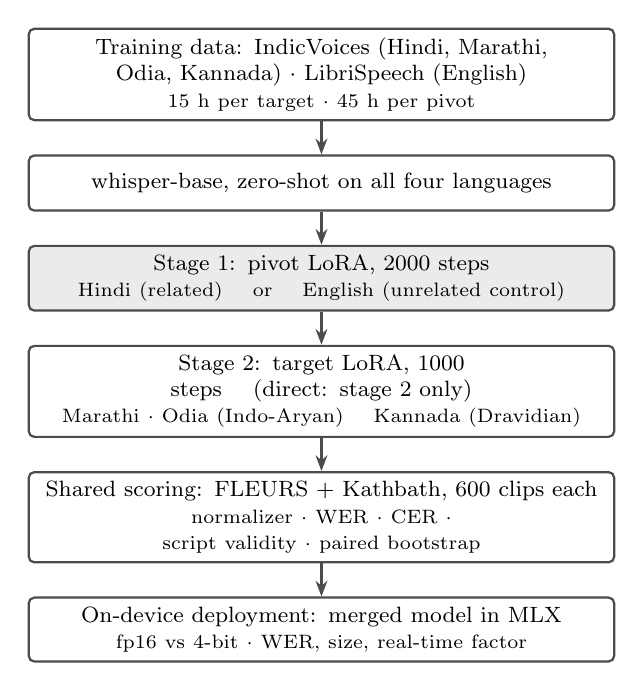
\begin{tikzpicture}[
  node distance=4.2mm,
  box/.style={rectangle, rounded corners=2pt, draw=black!70, thick,
              text width=7.2cm, align=center, minimum height=7mm,
              font=\footnotesize},
  ctrl/.style={box, fill=black!8},
  arrow/.style={-{Stealth[length=2mm]}, thick, draw=black!70}
]
\node[box] (data) {Training data: IndicVoices (Hindi, Marathi, Odia, Kannada) $\cdot$ LibriSpeech (English)\\ \scriptsize 15 h per target $\cdot$ 45 h per pivot};
\node[box, below=of data] (base) {whisper-base, zero-shot on all four languages};
\node[ctrl, below=of base] (pivot) {Stage 1: pivot LoRA, 2000 steps\\ \scriptsize Hindi (related) \quad or \quad English (unrelated control)};
\node[box, below=of pivot] (stage2) {Stage 2: target LoRA, 1000 steps \quad (direct: stage 2 only)\\ \scriptsize Marathi $\cdot$ Odia (Indo-Aryan) \quad Kannada (Dravidian)};
\node[box, below=of stage2] (eval) {Shared scoring: FLEURS + Kathbath, 600 clips each\\ \scriptsize normalizer $\cdot$ WER $\cdot$ CER $\cdot$ script validity $\cdot$ paired bootstrap};
\node[box, below=of eval] (deploy) {On-device deployment: merged model in MLX\\ \scriptsize fp16 vs 4-bit $\cdot$ WER, size, real-time factor};

\draw[arrow] (data) -- (base);
\draw[arrow] (base) -- (pivot);
\draw[arrow] (pivot) -- (stage2);
\draw[arrow] (stage2) -- (eval);
\draw[arrow] (eval) -- (deploy);
\end{tikzpicture}
\caption{The IndicBridge pipeline. Only the shaded stage varies: a related
(Hindi) or unrelated (English) pivot of equal size, or none.}
\label{fig:arch}
\end{figure}

% Generated by report/paper/build_assets.py from results/. Do not edit numbers by hand.
\begin{table}[!t]
\caption{Experimental Setup, Identical for Every Run}
\label{tab:setup}
\centering\scriptsize
\renewcommand{\arraystretch}{1.12}
\begin{tabular}{@{}p{1.55cm}p{6.35cm}@{}}
\hline
Base model & whisper-base (74M parameters), frozen\\
LoRA & $r{=}32$, $\alpha{=}64$, dropout 0.05, on $W_q$, $W_v$; 1.18M trainable\\
Optimiser & AdamW, lr $10^{-3}$, 100 warm-up steps, linear decay, grad.\ clip 1.0\\
Batch / precision & effective batch 16, fp32, seed 42\\
Steps & pivot 2000, target 1000\\
Hindi pivot & IndicVoices, 45 h, 19,127 clips, 1,474 speakers\\
English pivot & LibriSpeech clean-100, 45 h, 12,895 clips, 124 speakers\\
Marathi target & IndicVoices, 15 h, 6,141 clips, 721 speakers\\
Odia target & IndicVoices, 15 h, 7,227 clips, 1,150 speakers\\
Kannada target & IndicVoices, 15 h, 6,335 clips, 720 speakers\\
Clip filters & 2--30 s; $\le$50 clips per speaker; tagged rows dropped; labels $\le$443 tokens\\
Test sets & FLEURS test, Kathbath valid: 600 seeded clips each (Hindi FLEURS: all 417)\\
Decoding & greedy, no repetition penalty, length cap per language\\
Hardware & Apple M4, 16 GB unified memory, PyTorch (MPS)\\
\hline
\end{tabular}
\end{table}


\subsection{Data}

\WRITE{about 150 words: sources, filters, test sets, the decoder-length rule.}
% FACT: all training audio from IndicVoices \cite{javed2024indicvoices}
%       except English: LibriSpeech clean-100 \cite{panayotov2015librispeech}.
%       Clip and speaker counts are in Table II.     [data/train_*.json]
% FACT: filters, same for every language: clips 2-30 s; at most 50 clips
%       per speaker (English: 120, its speakers have long recordings);
%       rows whose text contains tags such as <unintelligible> dropped
%       (Hindi 1,044, Odia 704, Kannada 285, Marathi 157 rows); labels must
%       fit Whisper's decoder (<= 443 tokens; Odia lost 1,076 clips, Kannada
%       158 to this rule).                              [data/train_*.json]
% FACT: test sets never used for training: FLEURS test \cite{conneau2023fleurs}
%       and Kathbath valid \cite{javed2023indicsuperb}; a fixed seeded sample
%       of 600 clips each (Hindi FLEURS has only 417, all used).
% FACT: references longer than the decoder can write (440 tokens) are
%       excluded for every model: Odia FLEURS 202 of 875 (23.1%), Kannada
%       FLEURS 11 of 831 (1.3%), none elsewhere.        [data/test_*.json]

\subsection{Model and Training}

\WRITE{about 150 words: whisper-base, LoRA, the two stages.}
% FACT: base model whisper-base \cite{radford2023whisper} (74M parameters),
%       frozen. LoRA \cite{hu2022lora} on the query and value projections of
%       every attention block: 1.18M trainable parameters (1.6%).
%       [runs/H-odia/adapter: 72 tensors, 1,179,648 parameters]
% FACT: Eq. (1) is the LoRA update; r = 32, alpha = 64.
% FACT: multistage = stage 2 initialises from the pivot's adapter and keeps
%       training it on the target; direct = stage 2 from a fresh adapter.
% FACT: AdamW, lr 1e-3, 100 warm-up steps then linear decay to 0, gradient
%       clipping 1.0, effective batch 16, fp32, seed 42.
%       [runs/*/train_config.json, src/train_lora.py]
% FACT: implemented with Hugging Face Transformers \cite{wolf2020transformers}
%       and PEFT \cite{peft2022}; trained on an Apple M4 (16 GB) with
%       PyTorch MPS at 4.8-5.5 clips/s.             [runs/*/train_log.jsonl]
% FACT: why whisper-base: whisper-small trained at 1.35 clips/s on this
%       machine, making the grid ~99 h; whisper-base at ~4.5 clips/s.
%       [PLAN.md, measured]
\begin{equation}
W = W_0 + \frac{\alpha}{r} B A, \quad B \in \mathbb{R}^{d \times r},\; A \in \mathbb{R}^{r \times k}
\label{eq:lora}
\end{equation}

\subsection{Odia and the Borrowed Language Token}

\WRITE{about 80 words.}
% FACT: Whisper has no <|or|> token; every Odia run decodes under a borrowed
%       token: Bengali by default (closest relative with a token, fixed in
%       advance), plus Assamese and Hindi in the T runs and zero-shot.
% FACT: script validity, Eq. (3): share of output letters that fall in the
%       target language's Unicode script block.      [src/evaluate.py]

\subsection{Decoding, Normalization and Metrics}

\WRITE{about 130 words.}
% FACT: greedy decoding, no repetition penalty, identical for every run;
%       maximum new tokens = min(440, 10 + ceil(1.5 * r_L * s)) where s is
%       the clip length in seconds and r_L the fastest token rate observed
%       for language L (Hindi 19.0, Marathi 18.8, Kannada 26.0, Odia 43.7
%       tokens/s). Stops runaway loops without cutting real speech.
%       [src/eval_model.py, src/langs.py]
% FACT: one shared normalizer (contract v3.0.0) for every score: Unicode
%       NFC, annotation tags removed, Indic digits mapped to Western,
%       punctuation including danda and double danda removed, whitespace
%       collapsed. Vowel signs are kept (self-tested).  [src/normalize.py]
% FACT: three scores per run: raw, ours (normalized), and Whisper's own
%       BasicTextNormalizer, which replaces every Unicode mark (category M)
%       with a space -- in Indic scripts these are the vowel signs.
% FACT: WER and CER, Eq. (2); corpus level (total errors / total reference
%       words). Computed with jiwer.
% FACT: real-time factor RTF = decoding time / audio duration (Eq. 4).
\begin{equation}
\mathrm{WER} = \frac{S + D + I}{N} \times 100
\label{eq:wer}
\end{equation}
\begin{equation}
\mathrm{Script} = \frac{\#\{\text{letters in the target script}\}}{\#\{\text{letters}\}} \times 100
\label{eq:script}
\end{equation}
\begin{equation}
\mathrm{RTF} = t_{\mathrm{decode}} \,/\, t_{\mathrm{audio}}
\label{eq:rtf}
\end{equation}

\subsection{Statistical Testing}

\WRITE{about 120 words: the gains, the interaction, the bootstrap.}
% FACT: transfer gain of pivot p for target t, Eq. (5); Hindi-specific
%       gain Eq. (6); interaction Eq. (7).
% FACT: 95% intervals by paired bootstrap \cite{bisani2004bootstrap}:
%       1,000 resamples of test utterances; both systems scored on the same
%       resampled utterances; corpus-level WER recomputed per resample;
%       2.5th and 97.5th percentiles. Each comparison has its own fixed seed
%       so results do not depend on computation order. For the interaction,
%       each language's test set is resampled independently.
%       [src/analysis.py]
% FACT: "significant" here means the 95% interval excludes zero. One
%       training seed per configuration (state as a limitation).
\begin{equation}
G_p(t) = \mathrm{WER}_{\mathrm{direct}}(t) - \mathrm{WER}_{p \rightarrow t}(t), \quad p \in \{\mathrm{Hi}, \mathrm{En}\}
\label{eq:gain}
\end{equation}
\begin{equation}
\Delta(t) = G_{\mathrm{Hi}}(t) - G_{\mathrm{En}}(t) = \mathrm{WER}_{\mathrm{En} \rightarrow t} - \mathrm{WER}_{\mathrm{Hi} \rightarrow t}
\label{eq:delta}
\end{equation}
\begin{equation}
I(t_1, t_2) = \Delta(t_1) - \Delta(t_2)
\label{eq:interaction}
\end{equation}

\subsection{Deployment}

\WRITE{about 80 words.}
% FACT: each LoRA adapter merged into whisper-base and converted to MLX
%       \cite{mlx2023} (own converter; strict key check), fp16 (143.7 MB) and
%       4-bit (42.2 MB).                       [deploy/build_models.py]
% FACT: benchmark: 100 FLEURS clips per model, same clips scored by
%       PyTorch for reference; nothing else running on the GPU.
%       [deploy/bench_deploy.py]
% FACT: MLX decoding needed without_timestamps=True (the adapters were
%       trained with <|notimestamps|>) and Whisper's temperature fallback for
%       looping outputs, to match PyTorch accuracy.

\subsection{Native-Speaker Error Analysis}

\WRITE{about 80 words, only once the annotation sheets are filled.}
% FACT: 50 FLEURS test clips per language where at least one of the two
%       compared models made an error, drawn with a fixed seed (not hand
%       picked). Marathi/Odia/Kannada: direct vs Hindi multistage; Hindi:
%       zero-shot vs fine-tuned pivot.     [src/error_sample.py]
% FACT: categories: script, phonetic, morphology, segmentation,
%       code-switch, number, hallucination, reference wrong.
%       [results/error_analysis/README.md]

% ======================================================================
\section{Results and Insights}

% Generated by report/paper/build_assets.py from results/. Do not edit numbers by hand.
\begin{table}[!t]
\caption{WER and CER (\%) After Normalization. Best Per Language and Test Set in Bold}
\label{tab:main}
\centering\scriptsize
\setlength{\tabcolsep}{4pt}
\begin{tabular}{@{}llrrrr@{}}
\hline
 & & \multicolumn{2}{c}{FLEURS} & \multicolumn{2}{c}{Kathbath}\\
Language & Model & WER & CER & WER & CER\\
\hline
Hindi & Zero-shot & 154.7 & 134.8 & 137.0 & 115.3\\
 & Fine-tuned (pivot, 45 h) & \textbf{41.0} & \textbf{16.2} & \textbf{44.0} & \textbf{15.5}\\
\hline
Marathi & Zero-shot & 157.5 & 124.7 & 150.5 & 117.7\\
 & Direct & 63.4 & 20.5 & 67.1 & 21.4\\
 & Hindi $\rightarrow$ Marathi & \textbf{60.3} & \textbf{19.6} & \textbf{63.7} & \textbf{19.5}\\
 & English $\rightarrow$ Marathi & 63.3 & 20.4 & 68.3 & 21.0\\
\hline
Odia & Zero-shot & 194.2 & 166.3 & 184.2 & 150.3\\
 & Direct & 74.5 & 27.1 & 64.9 & 19.3\\
 & Hindi $\rightarrow$ Odia & \textbf{71.4} & \textbf{26.0} & \textbf{63.0} & \textbf{18.3}\\
 & English $\rightarrow$ Odia & 74.5 & 27.1 & 65.6 & 19.5\\
\hline
Kannada & Zero-shot & 192.5 & 140.1 & 210.7 & 150.2\\
 & Direct & 66.3 & 17.9 & 73.0 & 18.9\\
 & Hindi $\rightarrow$ Kannada & \textbf{65.2} & \textbf{17.6} & \textbf{72.2} & \textbf{18.5}\\
 & English $\rightarrow$ Kannada & 67.7 & 18.1 & 74.2 & 19.4\\
\hline
\end{tabular}
\end{table}


\subsection{Baseline and the Effect of Fine-Tuning}

\WRITE{about 110 words. Table~\ref{tab:main}.}
% FACT: zero-shot whisper-base WER is above 100% for every language (Hindi
%       154.7, Marathi 157.5, Kannada 192.5, Odia 194.2 on FLEURS): outputs
%       are longer than the reference and largely in the wrong script.
% FACT: zero-shot script validity: Odia 0%, Kannada 0%, Marathi 0.3%,
%       Hindi 7.4% (FLEURS); every fine-tuned model 100%.
%       [results/results_master.csv, column script_valid]
% FACT: Hindi fine-tuning (45 h): 154.7 -> 41.0 WER on FLEURS,
%       137.0 -> 44.0 on Kathbath.
% FACT: absolute WERs after training are high (60-75% on FLEURS) because
%       the model is whisper-base; the comparison between methods is the
%       result, not the absolute level.
% FACT: the Hindi-pivot model has the lowest WER and CER of all methods in
%       all six target/test-set cells (bold in Table III).

\subsection{Relatedness or Data Quantity?}

\WRITE{about 160 words: the main answer. Table~\ref{tab:gains}, Fig.~\ref{fig:gains}.}
% FACT (Table IV): Hindi pivot gain G_Hi significant for Marathi (+3.1,
%       +3.5) and Odia (+3.1, +1.9) on both test sets; Kannada +1.1 on
%       FLEURS (CI 0.1-2.3), +0.8 on Kathbath (CI includes zero).
% FACT: English pivot gain G_En never significantly positive; significantly
%       negative for Kannada on FLEURS (-1.3, CI -2.4 to -0.4).
% FACT: Delta (Hindi minus English) significantly positive in all six
%       cells: Marathi +3.0/+4.6, Odia +3.1/+2.6, Kannada +2.5/+1.9.
% FACT: CER shows the same direction: Hindi-specific CER gain positive and
%       significant in all six cells (Marathi +0.8/+1.5, Odia +1.1/+1.2,
%       Kannada +0.6/+0.9).                     [gains.csv, metric CER]
% INSIGHT to state in your words: the same hours and steps of English add
%       nothing, so the Hindi gain is not explained by data quantity or by
%       an extra training stage.
% CAVEAT (give it): the English stage moved the model less -- training loss
%       0.49 -> 0.08 and LoRA update norm 29.6, vs Hindi 1.31 -> 0.27 and
%       36.2 -- because Whisper is already strong in English, and LibriSpeech
%       audiobooks differ in domain from IndicVoices. [results/tables/pivots.csv]
% FACT: pivot-only models (no target training) write the target in the
%       wrong script: Hindi pivot on Odia 0% Odia script (148.8 WER).

\begin{figure}[!t]
\centering
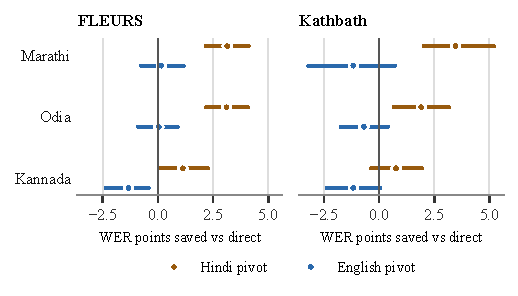
\includegraphics[width=\columnwidth]{figures/fig_gains.pdf}
\caption{Transfer gain over direct training (WER points; dot: gain, line:
95\% paired-bootstrap interval). An equal-size English pivot gives no gain;
the Hindi pivot helps every target.}
\label{fig:gains}
\end{figure}

% Generated by report/paper/build_assets.py from results/. Do not edit numbers by hand.
\begin{table}[!t]
\caption{Transfer Gains in WER Points With 95\% Paired-Bootstrap Intervals. Positive Means Fewer Errors; $\Delta = G_{\mathrm{Hi}} - G_{\mathrm{En}}$; Bold: Interval Excludes Zero}
\label{tab:gains}
\centering\scriptsize
\setlength{\tabcolsep}{2.2pt}
\begin{tabular}{@{}llccc@{}}
\hline
Target & Test & $G_{\mathrm{Hi}}$ & $G_{\mathrm{En}}$ & $\Delta$\\
\hline
Marathi & FLEURS & \textbf{+3.1} [2.2, 4.1] & +0.2 [$-$0.8, 1.2] & \textbf{+3.0} [2.1, 3.9]\\
 & Kathbath & \textbf{+3.5} [2.0, 5.2] & $-$1.2 [$-$3.2, 0.7] & \textbf{+4.6} [3.3, 6.4]\\
\hline
Odia & FLEURS & \textbf{+3.1} [2.2, 4.1] & 0.0 [$-$0.9, 0.9] & \textbf{+3.1} [2.1, 4.0]\\
 & Kathbath & \textbf{+1.9} [0.7, 3.2] & $-$0.7 [$-$1.8, 0.4] & \textbf{+2.6} [1.4, 3.9]\\
\hline
Kannada & FLEURS & \textbf{+1.1} [0.1, 2.3] & \textbf{$-$1.3} [$-$2.4, $-$0.4] & \textbf{+2.5} [1.4, 3.5]\\
 & Kathbath & +0.8 [$-$0.4, 2.0] & $-$1.2 [$-$2.4, 0.1] & \textbf{+1.9} [0.7, 3.2]\\
\hline
\end{tabular}
\end{table}


\subsection{Indo-Aryan Versus Dravidian Targets}

\WRITE{about 110 words: RQ1. Table~\ref{tab:interaction}.}
% FACT: FLEURS: no difference in Delta between any two targets (all three
%       intervals include zero).
% FACT: Kathbath: Marathi's Delta exceeds Kannada's by +2.7 (CI 1.0-4.8)
%       and Odia's by +2.0 (CI 0.1-4.3); Odia vs Kannada +0.7 (includes 0).
% INSIGHT: the benefit is "relatedness, but regional": an Indian pivot beats
%       an English one for every target, the Dravidian one included. A
%       family-specific extra is not consistent across test sets; where it
%       appears it is Marathi, which also shares Hindi's script.
% DO NOT CLAIM: that language family explains the gain.

% Generated by report/paper/build_assets.py from results/. Do not edit numbers by hand.
\begin{table}[!t]
\caption{Interaction: Difference in the Hindi-Specific Gain $\Delta$ Between Targets (WER Points, 95\% CI; Test Sets Resampled per Language)}
\label{tab:interaction}
\centering\scriptsize
\setlength{\tabcolsep}{4pt}
\begin{tabular}{@{}lcc@{}}
\hline
Comparison & FLEURS & Kathbath\\
\hline
$\Delta_{\mathrm{Mr}} - \Delta_{\mathrm{Kn}}$ & +0.5 [$-$1.0, 2.1] & \textbf{+2.7} [1.0, 4.8]\\
$\Delta_{\mathrm{Or}} - \Delta_{\mathrm{Kn}}$ & +0.6 [$-$0.8, 2.2] & +0.7 [$-$1.0, 2.4]\\
$\Delta_{\mathrm{Mr}} - \Delta_{\mathrm{Or}}$ & $-$0.1 [$-$1.4, 1.3] & \textbf{+2.0} [0.1, 4.3]\\
\hline
\end{tabular}
\end{table}


\subsection{Odia: Tokenizer Cost and the Borrowed Token}

\WRITE{about 120 words: RQ2. Table~\ref{tab:odia}.}
% FACT: Whisper spends 3.09 tokens per Odia letter (Hindi 1.29, Marathi
%       1.30, Kannada 1.89); 17.6 tokens per Odia word.  [fertility.csv]
% FACT: 23.1% of Odia FLEURS references (202 of 875) need more tokens than
%       Whisper's decoder can produce -- no model can transcribe them.
% FACT: zero-shot, every borrowed token gives 0% Odia script.
% FACT: after training, the token does not matter: Bengali 74.5/64.9,
%       Assamese 74.8/65.0, Hindi 73.8/64.6 WER (FLEURS/Kathbath). Hindi vs
%       Bengali: +0.7 (CI -0.1 to 1.6) FLEURS, +0.3 (CI -0.7 to 1.3)
%       Kathbath; Assamese vs Bengali: -0.4 (CI -1.1 to 0.5), -0.1 (CI -1.1
%       to 1.0). The genealogical order (Bengali/Assamese closest) does
%       not appear.                [report/paper/build_assets.py output]

% Generated by report/paper/build_assets.py from results/. Do not edit numbers by hand.
\begin{table}[!t]
\caption{Tokenizer Cost (FLEURS References) and the Borrowed Language Token for Odia}
\label{tab:odia}
\centering\scriptsize
\setlength{\tabcolsep}{3.5pt}
\begin{tabular}{@{}lrrr@{}}
\hline
Language & Tokens/letter & Tokens/word & Too long (\%)\\
\hline
Hindi & 1.29 & 5.18 & 0.0\\
Marathi & 1.30 & 7.60 & 0.0\\
Kannada & 1.89 & 13.87 & 1.3\\
Odia & 3.09 & 17.64 & 23.1\\
\hline
\end{tabular}

\vspace{4pt}
\begin{tabular}{@{}lccc@{}}
\hline
 & Zero-shot WER & Odia script & Trained WER\\
Token & FLEURS / Kathbath & (\%) & FLEURS / Kathbath\\
\hline
\texttt{<|bn|>} & 194.2 / 184.2 & 0 $\rightarrow$ 100 & 74.5 / 64.9\\
\texttt{<|as|>} & 199.3 / 182.5 & 0 $\rightarrow$ 100 & 74.9 / 65.0\\
\texttt{<|hi|>} & 210.3 / 230.6 & 0 $\rightarrow$ 100 & 73.8 / 64.6\\
\hline
\end{tabular}
\end{table}


\subsection{Effect of the Scoring Rules}

\WRITE{about 100 words: RQ3. Table~\ref{tab:norm}.}
% FACT: removing punctuation (ours vs raw) lowers FLEURS WER by 4.7-8.4 points across the nine trained models
%       (Marathi 68.7 -> 60.3); Kathbath references carry no punctuation,
%       so raw = ours there.
% FACT: Whisper's normalizer roughly halves WER (60.3 -> 30.5 Marathi
%       FLEURS) because it deletes vowel signs and splits words into
%       fragments; this score is not a valid measure for Indic scripts.
% FACT: with four methods ranked per target and test set, the Hindi-pivot
%       model is first under all three rules; Whisper's normalizer swaps the
%       direct and English-pivot models in 2 of 6 cases (Marathi Kathbath,
%       Odia FLEURS).

% Generated by report/paper/build_assets.py from results/. Do not edit numbers by hand.
\begin{table}[!t]
\caption{WER (\%) of the Hindi-Pivot Models Under Three Scoring Rules, and Whether the Ranking of the Four Methods Changes}
\label{tab:norm}
\centering\scriptsize
\setlength{\tabcolsep}{3.2pt}
\begin{tabular}{@{}llrrrc@{}}
\hline
Target & Test & Raw & Ours & Whisper & Order changes\\
\hline
Marathi & FLEURS & 68.7 & 60.3 & 30.5 & no\\
 & Kathbath & 63.7 & 63.7 & 29.5 & Whisper\\
Odia & FLEURS & 76.7 & 71.4 & 40.5 & Whisper\\
 & Kathbath & 62.9 & 63.0 & 30.1 & no\\
Kannada & FLEURS & 72.2 & 65.2 & 29.2 & no\\
 & Kathbath & 72.2 & 72.2 & 29.0 & no\\
\hline
\end{tabular}
\end{table}


\subsection{On-Device Deployment}

\WRITE{about 100 words. Table~\ref{tab:deploy}.}
% FACT: fp16 MLX, 144 MB: RTF 0.032-0.059 (17-31x faster than real time)
%       on the M4; WER within 2.5 points of PyTorch on the same clips
%       (largest gap Kannada 66.9 vs 64.4).
% FACT: 4-bit, 42 MB (3.4x smaller): WER 6-13 points worse; Kannada CER
%       rises from 17.0 to 72.1 -- quantisation breaks whisper-base for
%       Kannada. fp16 is the deployable choice.
% FACT: the demo runs the fp16 models fully offline (network off).

% Generated by report/paper/build_assets.py from results/. Do not edit numbers by hand.
\begin{table}[!t]
\caption{On-Device Deployment (MLX, Apple M4): 100 FLEURS Clips per Model. RTF = Decoding Time / Audio Duration}
\label{tab:deploy}
\centering\scriptsize
\setlength{\tabcolsep}{3.4pt}
\begin{tabular}{@{}llrrrrr@{}}
\hline
Model & Weights & MB & RTF & WER & CER & WER (PyTorch)\\
\hline
Hindi pivot & fp16 & 144 & 0.032 & 41.1 & 15.5 & 41.7\\
 & 4-bit & 42 & 0.022 & 47.7 & 19.5 & \\
Hi$\rightarrow$Mr & fp16 & 144 & 0.038 & 64.7 & 21.1 & 63.2\\
 & 4-bit & 42 & 0.025 & 70.8 & 24.0 & \\
Hi$\rightarrow$Or & fp16 & 144 & 0.059 & 72.0 & 27.0 & 71.7\\
 & 4-bit & 42 & 0.044 & 78.5 & 31.8 & \\
Hi$\rightarrow$Kn & fp16 & 144 & 0.058 & 66.9 & 17.0 & 64.4\\
 & 4-bit & 42 & 0.058 & 79.9 & 72.1 & \\
\hline
\end{tabular}
\end{table}


\subsection{Native-Speaker Error Analysis}

\WRITE{about 100 words, after running \texttt{report/paper/error\_tally.py} on the
filled sheets. Report which categories the Hindi pivot reduces and which
it does not. If the sheets are not complete, delete this subsection and
move the analysis to Future Scope.}
% \input{tables/errors}   % uncomment after error_tally.py writes it

\subsection{Limitations}

\WRITE{about 80 words.}
% FACT: one training seed per configuration (bootstrap intervals cover test
%       sampling, not training variance); whisper-base only; 600-clip test
%       samples; English pivot from a different domain (audiobooks) and
%       moved the model less; the Indo-Aryan targets include Marathi, which
%       shares Hindi's script, so script and family are not separated.

% ======================================================================
\section{Conclusion and Future Scope}

\WRITE{about 250 words: what was found (3-4 sentences), what it means for
choosing a pivot (1-2), future scope (3-4).}
% FACT (findings): see Sections VI-B to VI-F.
% FUTURE SCOPE -- things NOT done in this study (state them as future):
%   - a closer pivot for Odia (Marathi -> Odia) and a reversed family
%     mismatch (Kannada -> Odia), both planned in Review-1;
%   - a Dravidian pivot (e.g. Tamil or Telugu) to test family match from the
%     other side;
%   - several training seeds; larger Whisper models (small, medium);
%   - separating script from family (e.g. a Devanagari vs non-Devanagari
%     Indo-Aryan target);
%   - a tokenizer that does not split Odia letters into bytes;
%   - native-speaker error analysis (if not completed).

% ======================================================================
\begin{thebibliography}{24}

\bibitem{conneau2021xlsr}
A. Conneau, A. Baevski, R. Collobert, A. Mohamed, and M. Auli,
``Unsupervised Cross-Lingual Representation Learning for Speech
Recognition,'' in \emph{Proc. INTERSPEECH}, 2021, pp. 2426--2430.

\bibitem{babu2022xlsr}
A. Babu, C. Wang, A. Tjandra, K. Lakhotia, Q. Xu, N. Goyal,
K. Singh, P. von Platen, Y. Saraf, J. Pino, A. Baevski, A. Conneau, and
M. Auli, ``XLS-R: Self-Supervised Cross-Lingual Speech Representation
Learning at Scale,'' in \emph{Proc. INTERSPEECH}, 2022, pp. 2278--2282.

\bibitem{radford2023whisper}
A. Radford, J. W. Kim, T. Xu, G. Brockman, C. McLeavey, and
I. Sutskever, ``Robust Speech Recognition via Large-Scale Weak
Supervision,'' in \emph{Proc. International Conference on Machine
Learning (ICML)}, 2023, pp. 28492--28518.

\bibitem{pratap2024mms}
V. Pratap, A. Tjandra, B. Shi, P. Tomasello, A. Babu, S. Kundu,
A. Elkahky, Z. Ni, A. Vyas, M. Fazel-Zarandi, A. Baevski, Y. Adi,
X. Zhang, W.-N. Hsu, A. Conneau, and M. Auli, ``Scaling Speech
Technology to 1{,}000+ Languages,'' \emph{Journal of Machine Learning
Research}, vol. 25, no. 97, pp. 1--52, 2024.

\bibitem{rouditchenko2023unseen}
A. Rouditchenko, S. Khurana, S. Thomas, R. Feris, L. Karlinsky,
H. Kuehne, D. Harwath, B. Kingsbury, and J. Glass, ``Comparison of
Multilingual Self-Supervised and Weakly-Supervised Speech Pre-Training
for Adaptation to Unseen Languages,'' in \emph{Proc. INTERSPEECH}, 2023,
pp. 2268--2272.

\bibitem{pillai2024multistage}
L. G. Pillai, K. Manohar, B. K. Raju, and E. Sherly, ``Multistage
Fine-tuning Strategies for Automatic Speech Recognition in Low-resource
Languages,'' \emph{ACM Transactions on Asian and Low-Resource Language
Information Processing}, vol. 25, no. 8, pp. 1--12, 2026,
doi: 10.1145/3813800.

\bibitem{hu2022lora}
E. J. Hu, Y. Shen, P. Wallis, Z. Allen-Zhu, Y. Li, S. Wang, L. Wang, and
W. Chen, ``LoRA: Low-Rank Adaptation of Large Language Models,'' in
\emph{Proc. International Conference on Learning Representations
(ICLR)}, 2022.

\bibitem{houlsby2019adapters}
N. Houlsby, A. Giurgiu, S. Jastrzebski, B. Morrone, Q. de Laroussilhe,
A. Gesmundo, M. Attariyan, and S. Gelly, ``Parameter-Efficient Transfer
Learning for NLP,'' in \emph{Proc. International Conference on Machine
Learning (ICML)}, 2019, pp. 2790--2799.

\bibitem{pfeiffer2020madx}
J. Pfeiffer, I. Vuli\'{c}, I. Gurevych, and S. Ruder, ``MAD-X: An
Adapter-Based Framework for Multi-Task Cross-Lingual Transfer,'' in
\emph{Proc. Empirical Methods in Natural Language Processing (EMNLP)},
2020, pp. 7654--7673.

\bibitem{song2024lorawhisper}
Z. Song, J. Zhuo, Y. Yang, Z. Ma, S. Zhang, and X. Chen, ``LoRA-Whisper:
Parameter-Efficient and Extensible Multilingual ASR,'' in \emph{Proc.
INTERSPEECH}, 2024, pp. 3934--3938.

\bibitem{xu2024rehearsalfree}
T. Xu, K. Huang, P. Guo, Y. Zhou, L. Huang, H. Xue, and L. Xie,
``Towards Rehearsal-Free Multilingual ASR: A LoRA-Based Case Study on
Whisper,'' in \emph{Proc. INTERSPEECH}, 2024, pp. 2534--2538.

\bibitem{ferraz2024distilwhisper}
T. P. Ferraz, M. Z. Boito, C. Brun, and V. Nikoulina, ``Multilingual
DistilWhisper: Efficient Distillation of Multi-Task Speech Models via
Language-Specific Experts,'' in \emph{Proc. IEEE International
Conference on Acoustics, Speech and Signal Processing (ICASSP)}, 2024,
pp. 10716--10720.

\bibitem{bhogale2023vistaar}
K. S. Bhogale, S. Sundaresan, A. Raman, T. Javed, M. M. Khapra, and
P. Kumar, ``Vistaar: Diverse Benchmarks and Training Sets for Indian
Language ASR,'' in \emph{Proc. INTERSPEECH}, 2023, pp. 4384--4388.

\bibitem{javed2024indicvoices}
T. Javed, J. Nawale, E. George, S. Joshi, K. Bhogale, D. Mehendale,
I. Sethi, \emph{et al.},
``IndicVoices: Towards Building an Inclusive Multilingual Speech Dataset
for Indian Languages,'' in \emph{Findings of the Association for
Computational Linguistics: ACL}, 2024, pp. 10740--10782.

\bibitem{javed2023indicsuperb}
T. Javed, K. S. Bhogale, A. Raman, P. Kumar, A. Kunchukuttan, and
M. M. Khapra, ``IndicSUPERB: A Speech Processing Universal Performance
Benchmark for Indian Languages,'' in \emph{Proc. AAAI Conference on
Artificial Intelligence}, vol. 37, no. 11, 2023, pp. 12942--12950.

\bibitem{conneau2023fleurs}
A. Conneau, M. Ma, S. Khanuja, Y. Zhang, V. Axelrod, S. Dalmia,
J. Riesa, C. Rivera, and A. Bapna, ``FLEURS: Few-Shot Learning
Evaluation of Universal Representations of Speech,'' in \emph{Proc. IEEE
Spoken Language Technology Workshop (SLT)}, 2023, pp. 798--805.

\bibitem{ardila2020commonvoice}
R. Ardila, M. Branson, K. Davis, M. Kohler, J. Meyer, M. Henretty,
R. Morais, L. Saunders, F. M. Tyers, and G. Weber, ``Common Voice: A
Massively-Multilingual Speech Corpus,'' in \emph{Proc. Language
Resources and Evaluation Conference (LREC)}, 2020, pp. 4218--4222.

\bibitem{pineiro2024weighted}
A. Pi\~{n}eiro-Mart\'{i}n, C. Garc\'{i}a-Mateo, L. Doc\'{i}o-Fern\'{a}ndez,
M. del Carmen L\'{o}pez-P\'{e}rez, and G. Rehm, ``Weighted
Cross-Entropy for Low-Resource Languages in Multilingual Speech
Recognition,'' in \emph{Proc. INTERSPEECH}, 2024, pp. 1235--1239.

\bibitem{panayotov2015librispeech}
V. Panayotov, G. Chen, D. Povey, and S. Khudanpur, ``Librispeech: An
ASR Corpus Based on Public Domain Audio Books,'' in \emph{Proc. IEEE
International Conference on Acoustics, Speech and Signal Processing
(ICASSP)}, 2015, pp. 5206--5210.

\bibitem{bisani2004bootstrap}
M. Bisani and H. Ney, ``Bootstrap Estimates for Confidence Intervals in
ASR Performance Evaluation,'' in \emph{Proc. IEEE International
Conference on Acoustics, Speech and Signal Processing (ICASSP)}, vol. 1,
2004, pp. I-409--I-412.

\bibitem{wolf2020transformers}
T. Wolf, L. Debut, V. Sanh, J. Chaumond, C. Delangue, A. Moi,
P. Cistac, T. Rault, R. Louf, M. Funtowicz, \emph{et al.},
``Transformers: State-of-the-Art Natural Language Processing,'' in
\emph{Proc. EMNLP: System Demonstrations}, 2020, pp. 38--45.

\bibitem{peft2022}
S. Mangrulkar, S. Gugger, L. Debut, Y. Belkada, S. Paul, B. Bossan, and
M. Tietz, ``PEFT: State-of-the-Art Parameter-Efficient Fine-Tuning
Methods,'' 2022. [Online]. Available: \url{https://github.com/huggingface/peft}

\bibitem{mlx2023}
A. Hannun, J. Digani, A. Katharopoulos, and R. Collobert, ``MLX:
Efficient and Flexible Machine Learning on Apple Silicon,'' 2023.
[Online]. Available: \url{https://github.com/ml-explore/mlx}

\end{thebibliography}

\end{document}
